\documentclass[10pt]{article}
\usepackage[ngerman]{babel}
\usepackage[utf8]{inputenc}
\usepackage[T1]{fontenc}
\usepackage{graphicx}
\usepackage[export]{adjustbox}
\graphicspath{ {./images/} }
\usepackage{amsmath}
\usepackage{amsfonts}
\usepackage{amssymb}
\usepackage[version=4]{mhchem}
\usepackage{stmaryrd}

\title{Bachelor of Science (BSc) in Informatik Modul Software-Entwicklung 1 (SWEN1) }

\author{}
\date{}


\begin{document}
\maketitle
\section*{V1 - Verteilte Systeme}
SWEN1/PM3 Team:\\
R. Ferri (feit), D. Liebhart (lieh), K. Bleisch (bles), G. Wyder (wydg)

\section*{Um was geht es?}
\begin{itemize}
  \item Was sind verteilte Systeme?
  \item Wie ist der prinzipielle Aufbau eines Client-Server-Systems?
  \item Welche Phänomene und Probleme ergeben sich bei verteilten Systemen?
  \item Welche Aspekte sind zu berücksichtigen beim Design und der Implementierung eines Client-Server-Systems?
  \item Was sind gängige Technologien (Middleware)\\

\includegraphics[width=\linewidth]{images/2025_01_02_9418c7c99690de3f1353g-02(1)} zur Entwicklung von verteilten Systemen?\\
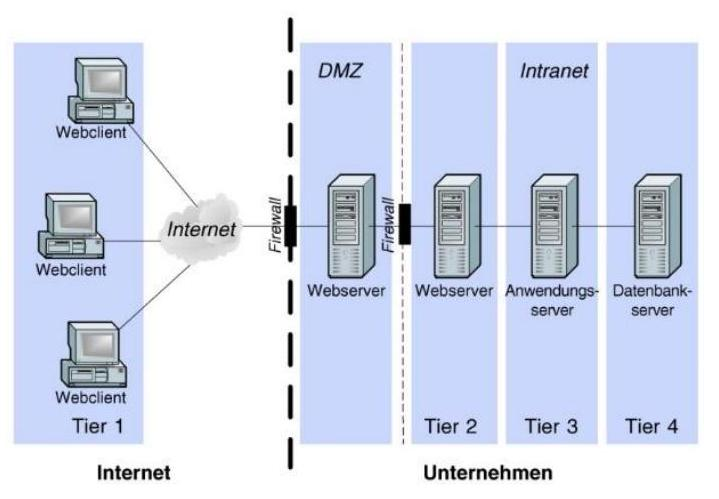
\includegraphics[width=\linewidth]{images/2025_01_02_9418c7c99690de3f1353g-02}
\end{itemize}

\section*{Lernziele VT 01 - Verteilte Systeme}
Sie sind in der Lage,

\begin{itemize}
  \item zu erläutern, was ein verteiltes System ist und warum verteilte Systeme eingesetzt werden,
  \item die fundamentalen Konzepte eines verteilten Systems wie Architekturstil, Kommunikationsverfahren, Fehlertoleranz und Fehlersemantik zu erläutern,
  \item wichtige Design- und Implementierungsaspekte von Client-Server-Systemen zu diskutieren,
  \item für einen Entwurf eines verteilten Systems gängige Architektur und Design Patterns zu benutzen,
  \item gängige Technologien (Middleware) zur Entwicklung von verteilten betrieblichen Informationssystemen und Internet-basierten Systemen einzuordnen.
\end{itemize}

\begin{enumerate}
  \item Einführung in verteilte Systeme
  \item Design- und Implementierungskonzepte von Client-Server-Systemen
  \item Middleware für verteilte Systeme
  \item Wrap-up und Ausblick
\end{enumerate}

\section*{Was ist ein verteiltes System?}
\section*{- Verteiltes System}
\begin{itemize}
  \item Basiert auf einer Menge voneinander unabhängiger Rechnersysteme (Knoten) und Softwarebausteinen (Komponenten).
  \item Erscheinen dem Benutzer wie ein einzelnes, kohärentes System bzw. Anwendungssystem.
\end{itemize}

\section*{- Verteilte Anwendung}
\begin{itemize}
  \item Anwendung, die auf einem verteilten System läuft.
  \item Jeder Softwarebaustein kann auf einem eigenen Rechner liegen.
  \item Es können aber auch mehrere Softwarebausteine auf dem gleichen Rechner installiert sein.
\end{itemize}

\section*{Historische Entwicklung}
Verteilte Systeme\\
Client/Server-Computing\\
Personal\\
Computer\\
Timesharing-\\
Systeme\\
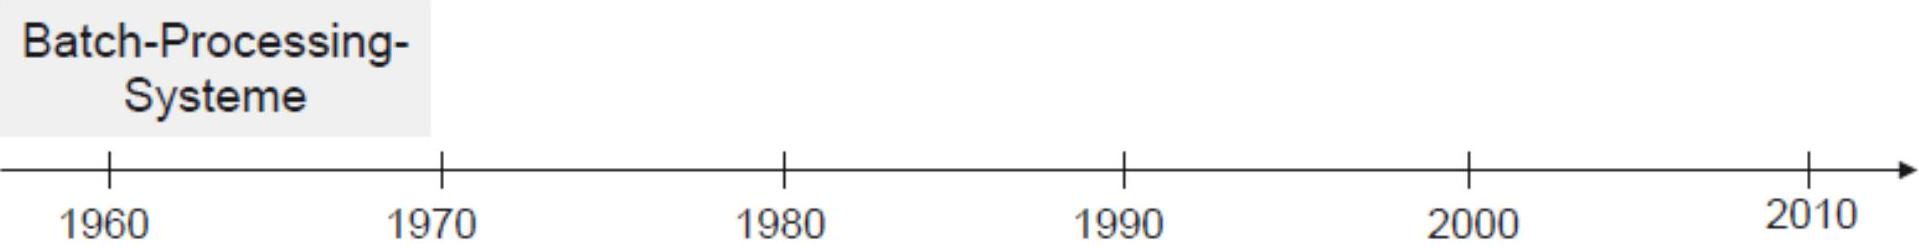
\includegraphics[width=\linewidth]{images/2025_01_02_9418c7c99690de3f1353g-06}

Die folgenden Faktoren haben die Entwicklung wesentlich beeinflusst:

\begin{itemize}
  \item Leistungsexplosion in der Mikroprozessortechnik,
  \item schnelle lokale Netzwerke (LAN)
  \item Verbindung mehrerer physischer Netze zu einem einheitlichen Kommunikationssystem (WAN) und das Anbieten eines Universaldienstes für heterogene Netzwerke, dem Internet
\end{itemize}

\section*{Typische verteilte Systeme heute sind...}
\begin{itemize}
  \item Informationssysteme
  \item Mobile Systeme
  \item Eingebettete Systeme
  \item Cloudbasierte Systeme
  \item Hochleistungsrechnersysteme\\
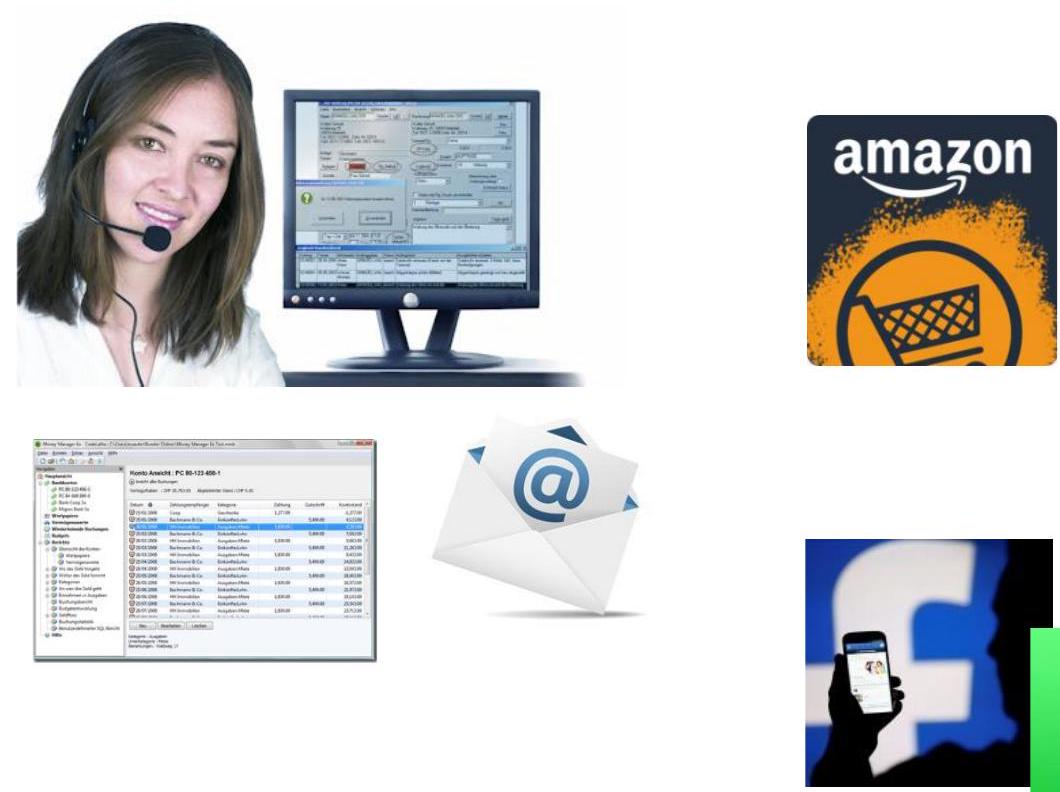
\includegraphics[width=\linewidth]{images/2025_01_02_9418c7c99690de3f1353g-07(1)}\\
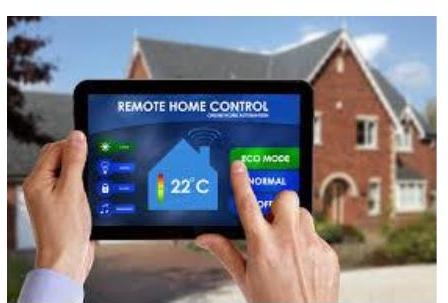
\includegraphics[width=\linewidth]{images/2025_01_02_9418c7c99690de3f1353g-07}
\end{itemize}

\section*{Was sind verteilte Informationssysteme?}
\begin{itemize}
  \item Verteilte Informationssysteme sind verteilte Systeme mit besonderen Merkmalen.
  \item Typische Merkmale:
  \item Oft sehr gross
  \item Sehr datenorientiert: Datenbanken im Zentrum der Anwendung
  \item Extrem interaktiv: GUI, aber auch Batch
  \item Sehr nebenläufig: Grosse Anzahl an parallel arbeitenden Benutzern
  \item Oft hohe Konsistenzanforderungen
\end{itemize}

\section*{Warum setzt man auf verteilte Systeme?}
\begin{itemize}
  \item Vorteile:
  \item Gemeinsamer Ressourcenzugriff
  \item Lastverteilung
  \item Ausfallsicherheit, Verfügbarkeit
  \item Skalierbarkeit
  \item Flexibilität
  \item Verteilungstransparenz (Ort, Fehler, Persistenz, ...)
  \item Nachteile:
  \item Komplexität durch Verteilung, Netzinfrastruktur\\
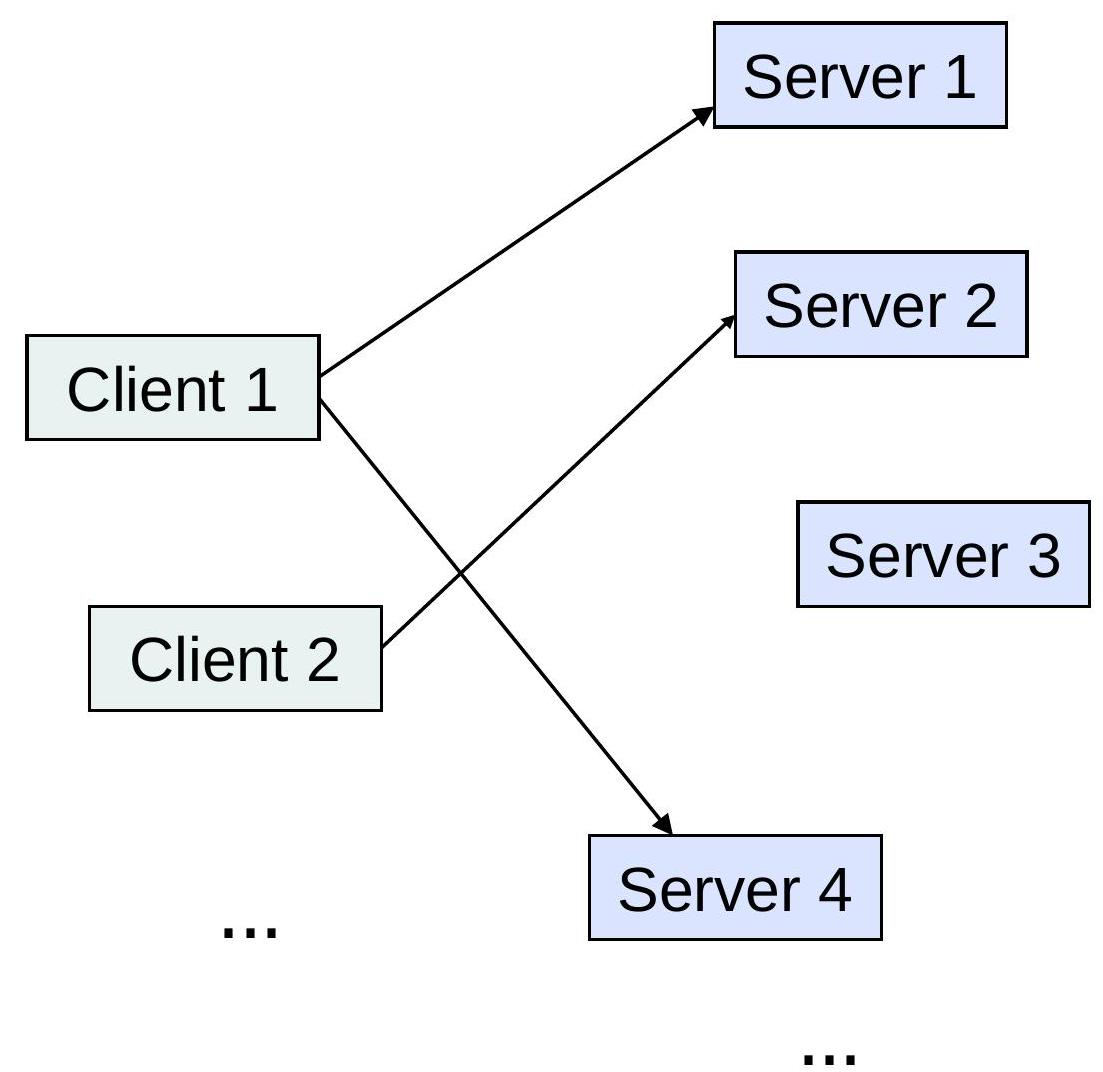
\includegraphics[width=\linewidth]{images/2025_01_02_9418c7c99690de3f1353g-09}
\end{itemize}

\section*{Architekturmodelle verteilter Systeme}
\begin{itemize}
  \item Ein Architekturmodell beschreibt die Rollen der Komponenten innerhalb einer verteilten Anwendung sowie die Beziehungen zwischen innen.
  \item Heute finden vor allem folgende Architekturmodelle ihren Einsatz:
\end{itemize}

\section*{Client/Server}
\begin{center}
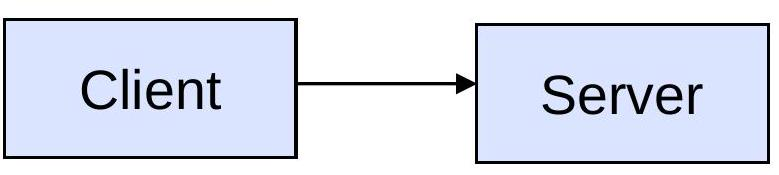
\includegraphics[width=\linewidth]{images/2025_01_02_9418c7c99690de3f1353g-10}
\end{center}

Kurzlebiger Client-Prozess, der mit einem langlebigen Server-Prozess kommuniziert (z.B. Web-Applikation)

Peer-to-Peer\\
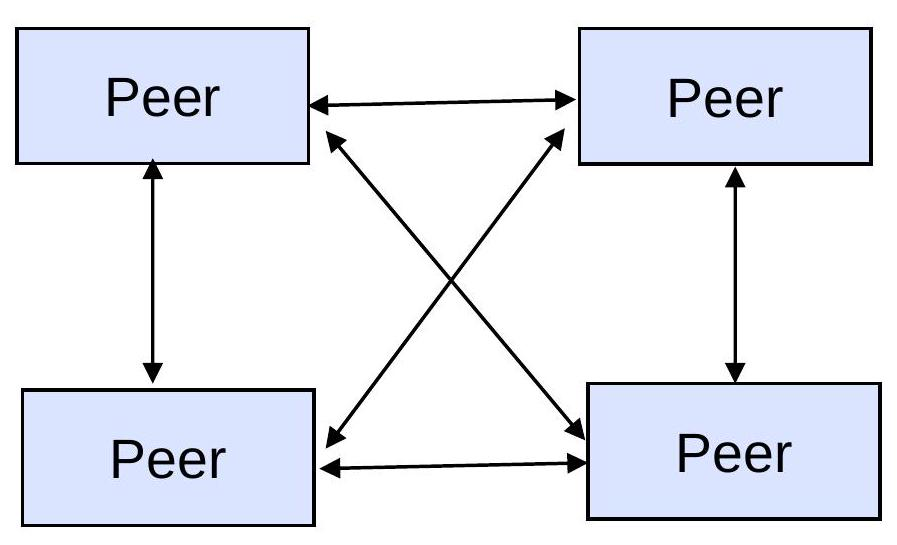
\includegraphics[width=\linewidth]{images/2025_01_02_9418c7c99690de3f1353g-10(2)}

Gleichberechtigte Peer-Prozesse, die nur bei Bedarf Informationen austauschen (z.B. Blockchain)

VT 01 - Verteilte Systeme | Ausgabe HS24

Event Systems\\
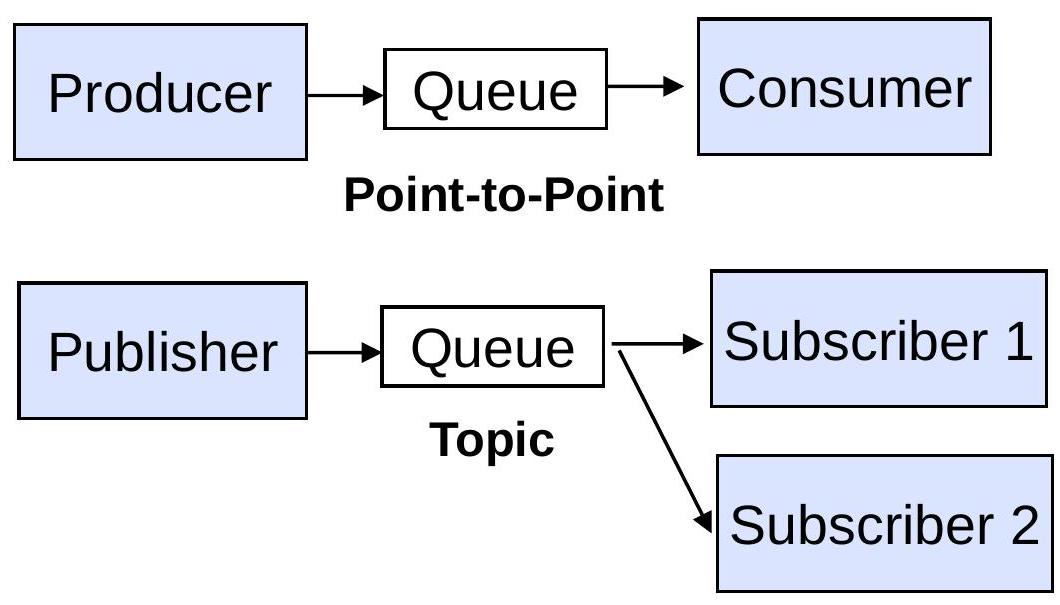
\includegraphics[width=\linewidth]{images/2025_01_02_9418c7c99690de3f1353g-10(1)}

Event-Sources-Prozesse und Event-Sinks-Prozesse, die asynchron Informationen austauschen (z.B. E-Mail)

\section*{Mehrstufige Architekturen (Multi-Tier-Architekturen)}
\begin{itemize}
  \item Multi-Tier-Architekturen sind eine Ergänzung zum Client-Server-Architekturmodell und beschreiben Modelle zur Verteilung einer Anwendung auf den Rechnern (engl. tiers) des verteilten Systems.
  \item Für die Arbeitsteilung zwischen Client und Server existieren verschiedene Alternativen, je nachdem, wo die Schichten (Layer) Präsentation, Verarbeitung (Domänenlogik) und Datenhaltung angesiedelt sind.\\
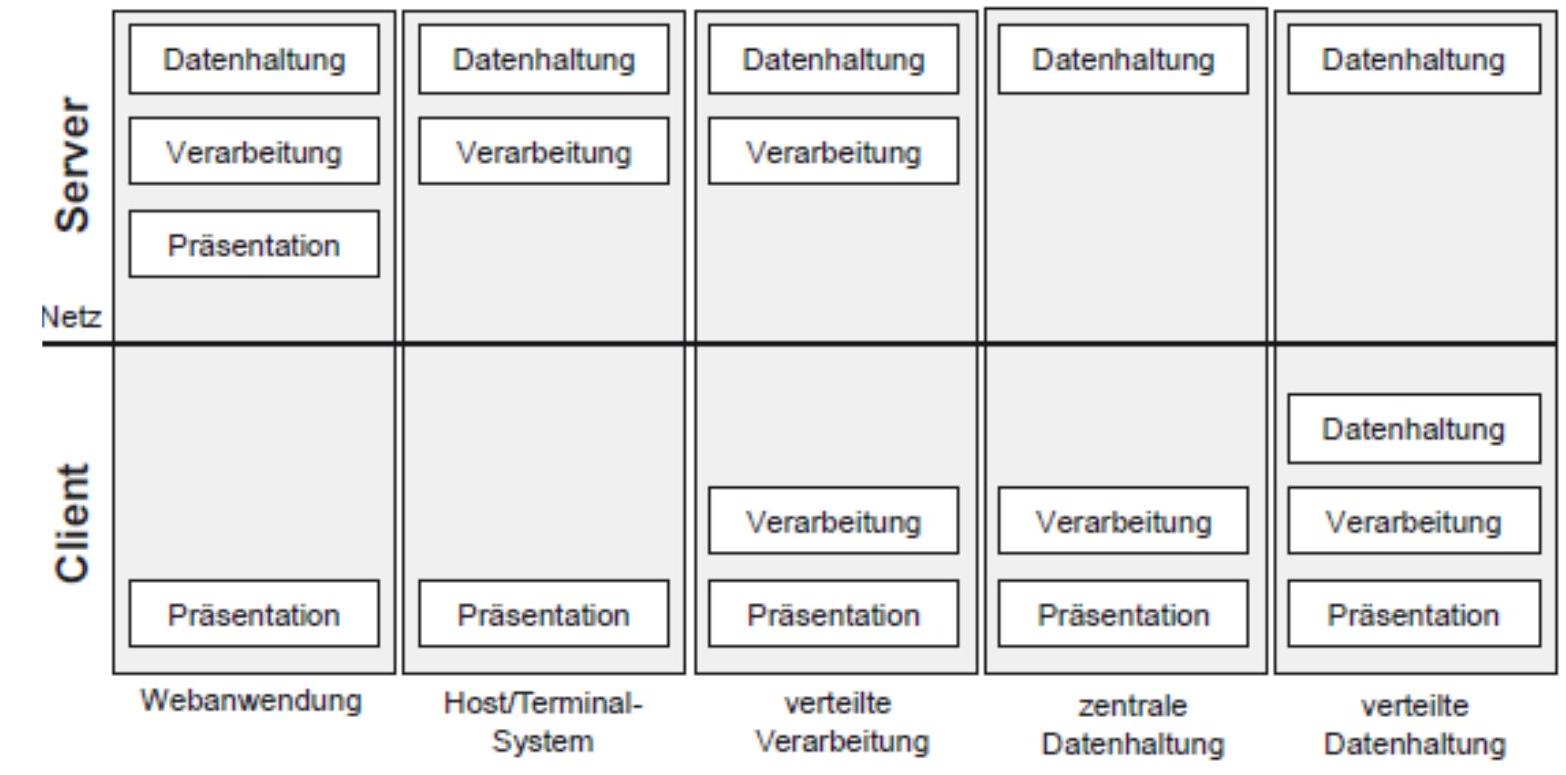
\includegraphics[width=\linewidth]{images/2025_01_02_9418c7c99690de3f1353g-11(1)}
\end{itemize}

Beispiel: 3-Tier-Architektur\\
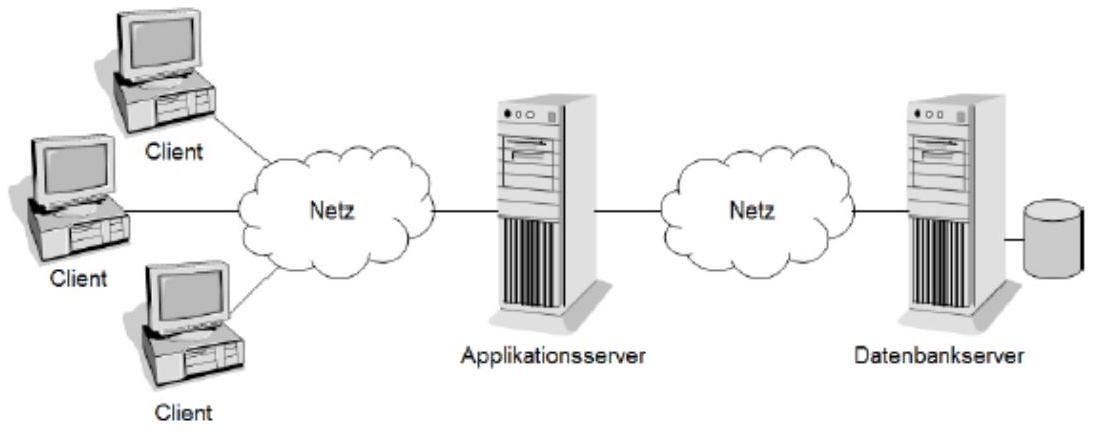
\includegraphics[width=\linewidth]{images/2025_01_02_9418c7c99690de3f1353g-11}

\begin{enumerate}
  \item Einführung in verteilte Systeme
  \item Design- und Implementierungskonzepte von Client-Server-Systemen
  \item Middleware für verteilte Systeme
  \item Wrap-up und Ausblick
\end{enumerate}

\section*{Terminologie bzw. Metamodell für die Diskussion von Client-Server-Systemen}
\begin{itemize}
  \item Ein Server stellt eine Ablaufumgebung für einen oder mehrere Serverbausteine bereit.
  \item Ein Applikationsserver ist auch ein Server, auf dem Serverbausteine ausgeführt werden, aber im engeren Sinne noch verschiedene Dienste den Serverbausteinen anbietet (z.B. Authentifizierung, Transaktionen etc.).
  \item Ein Serverbaustein ist ein Objekt, Modul oder Komponente (je nach verwendetem Programmiermodell), das zum Ablaufzeitpunkt instanziiert und bei Bedarf einem Client für die Abarbeitung einer Anforderung (eines\\
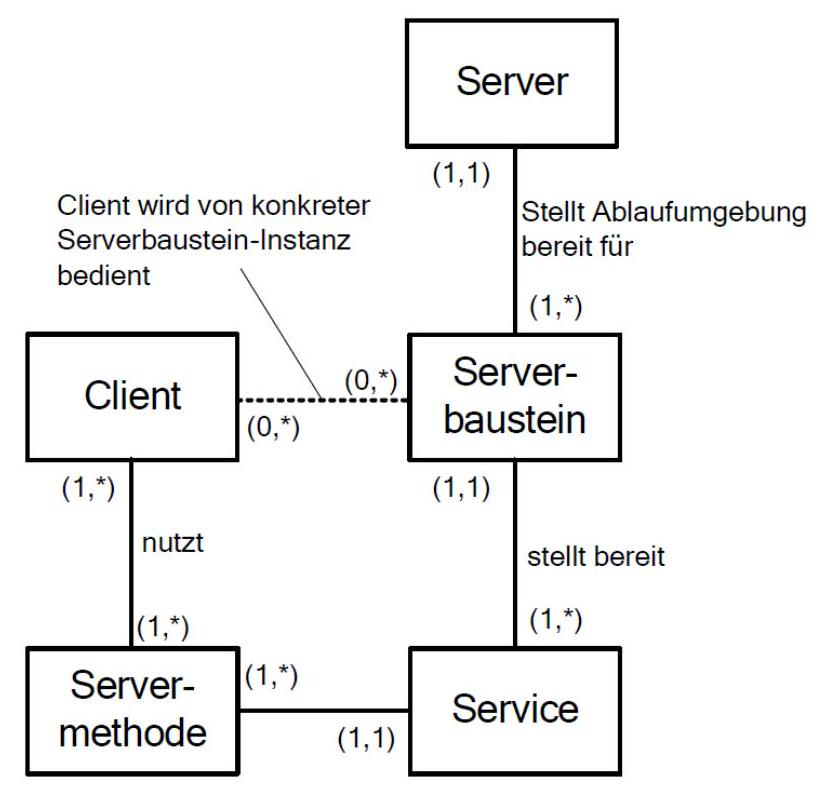
\includegraphics[width=\linewidth]{images/2025_01_02_9418c7c99690de3f1353g-13} Requests) zugeordnet wird.
  \item Ein Service oder Dienst wird durch einen Serverbaustein bereitgestellt und enthält eine oder mehrere Servermethoden oder Serverprozeduren.
  \item Eine Servermethode oder eine Serverprozedur ist Bestandteil eines Services, den ein Client durch das Senden eines entsprechenden Requests nutzen kann.
\end{itemize}

\section*{Kommunikation zwischen Client und Server (1/2)}
\begin{itemize}
  \item Jeder Service ist über seine URL aufrufbar:
  \item protokoll://<server>:<port>/<pfad\_des\_service>
  \item Kommunikation zwischen Client und Server
  \item Über TCP oder UDP
  \item Socket
  \item Programmierschnittstelle zu Kommunikationskanal
  \item IP-Socket-Adresse: IP-Adresse + Portnummer\\
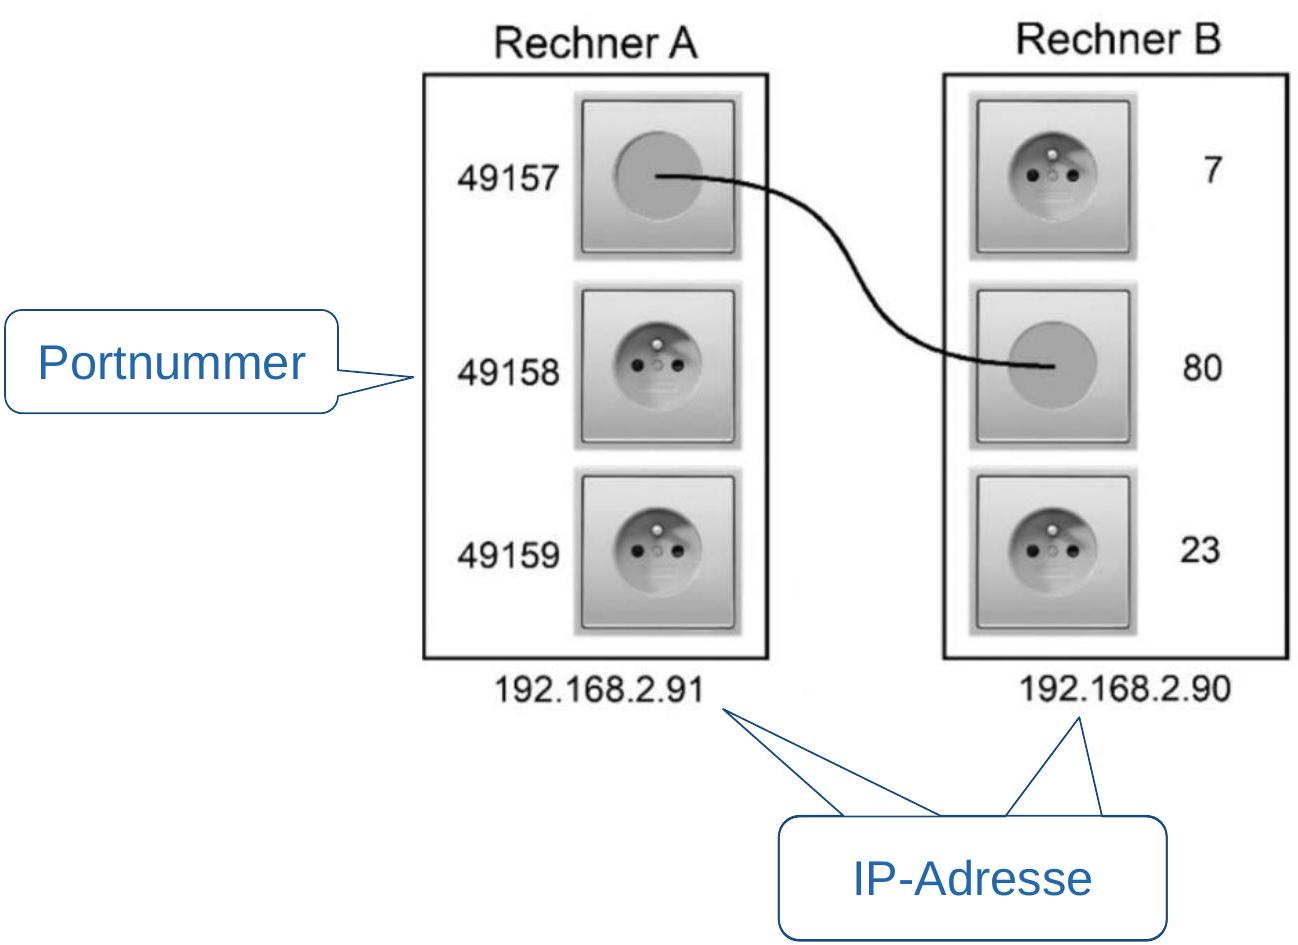
\includegraphics[width=\linewidth]{images/2025_01_02_9418c7c99690de3f1353g-14}
\end{itemize}

\section*{Kommunikation zwischen Client und Server (2/2)}
\begin{itemize}
  \item Client sendet Request an Server
  \item Ein Server empfängt den Client-Request und leitet diesen zur Verarbeitung an den entsprechenden Service (des betreffenden Serverbausteins) weiter.
  \item Service bearbeitet Request und schickt Antwort (Response) zurück an den Client.
  \item Ein Server ist seinerseits in eine Ablaufumgebung (z.B. VM)\\
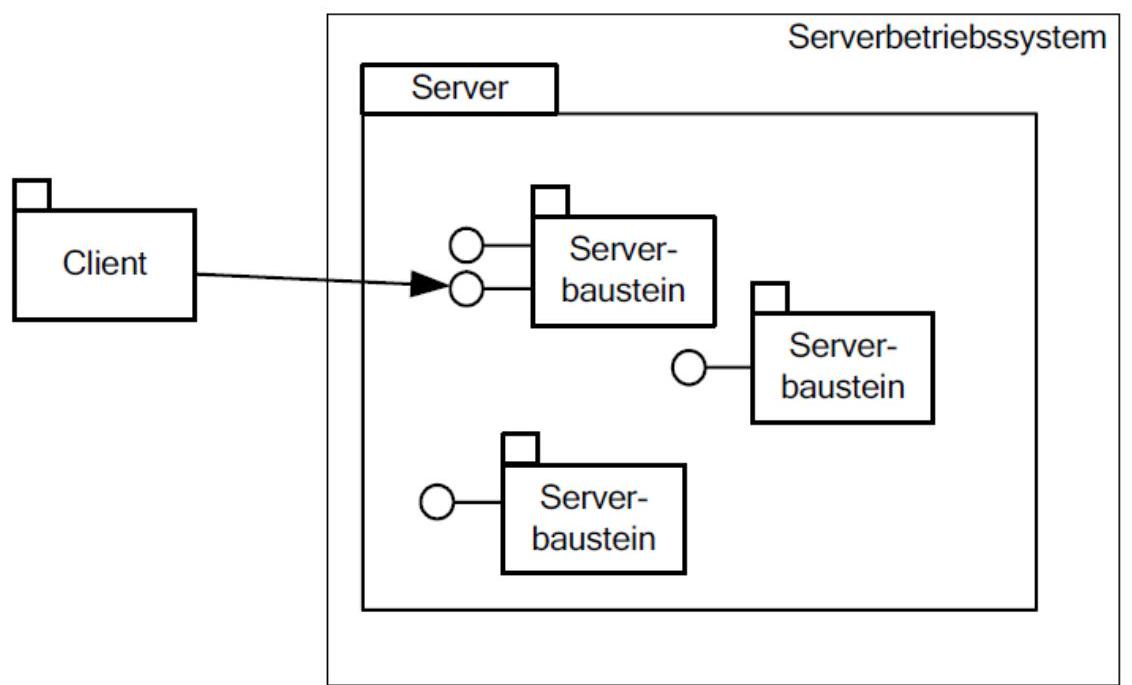
\includegraphics[width=\linewidth]{images/2025_01_02_9418c7c99690de3f1353g-15} innerhalb des Rechnerbetriebssystems eingebettet.
  \item Server und Serverbaustein müssen vor der Verwendung instanziiert werden.
\end{itemize}

\section*{Lebenszyklus von Serverbausteinen}
\begin{itemize}
  \item Ein Serverbaustein wird zur Laufzeit von einem Server instanziiert und durchläuft, je nach Bausteintyp und Implementierung verschiedene Zustände.
  \item Zustandsdiagramm für eine Serverbaustein-Instanz:\\
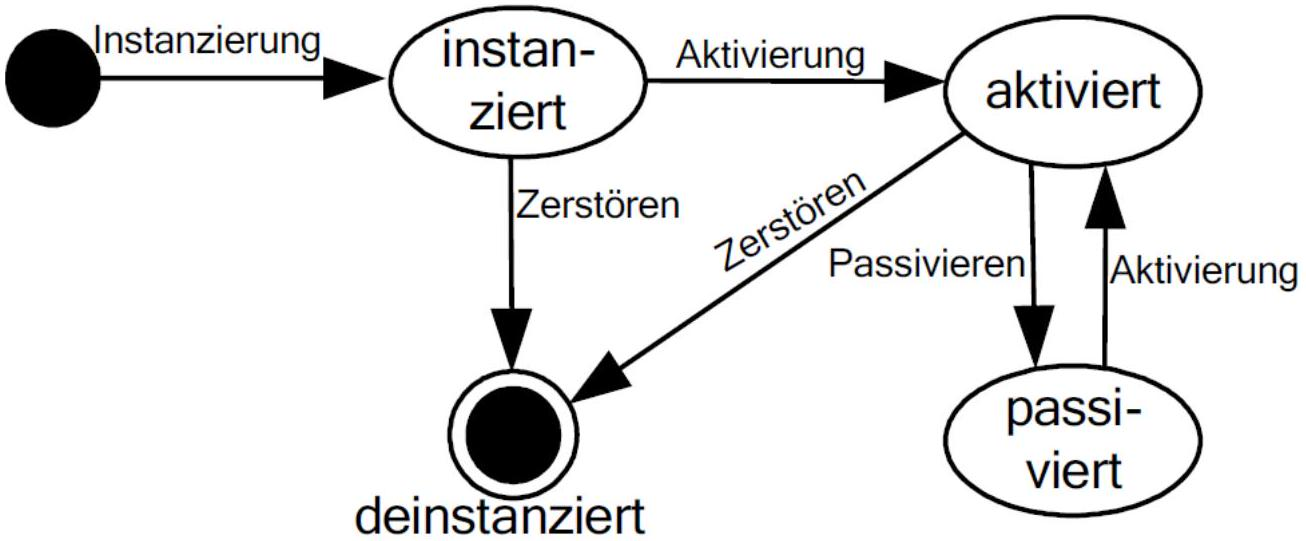
\includegraphics[width=\linewidth]{images/2025_01_02_9418c7c99690de3f1353g-16}
  \item Die Anzahl und Benennung der Zustände sind je nach Client-Server-Implementierung (Middleware) verschieden.
\end{itemize}

\section*{Verwendetes Design Pattern für den Zugriff auf Services in Serverbausteinen}
School of Engineering InIT Institut für angewandt Informationstechnologie

\begin{itemize}
  \item Grundlegendes Design Pattern für den Zugriff auf Serverbausteine ist das Remote Proxy.\\
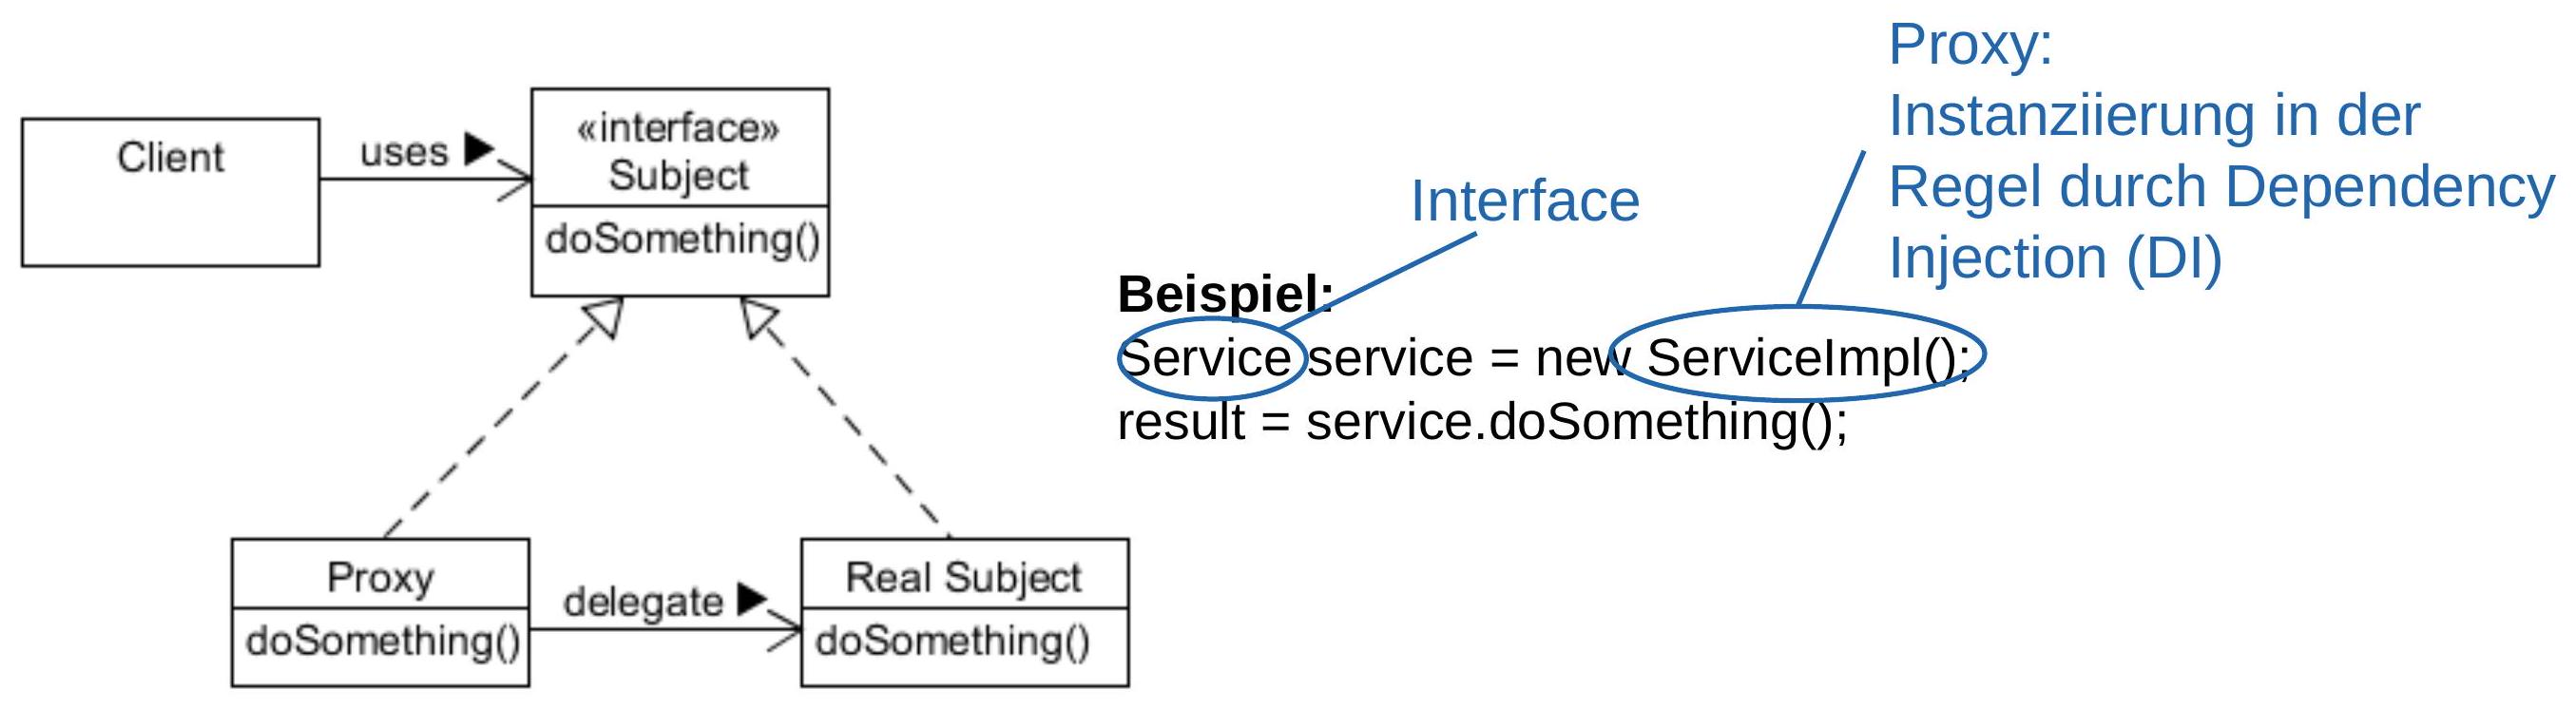
\includegraphics[width=\linewidth]{images/2025_01_02_9418c7c99690de3f1353g-17}
\end{itemize}

Service service $=$ new Servicelmpl().\\
result = service.doSomething();

Anmerkung: In einer Client-Server-Implementierung heisst der (client- und serverseitige) Proxy auch Stub (von englisch stub, Stubben, Stummel, Stumpf). Ein server-seitig generierter Stub wird dabei Skeleton (engl. Skelett, Gerippe, Gerüst) genannt.

\section*{Verwendetes Design Pattern für den Datenaustausch zwischen Client und Server}
\begin{itemize}
  \item Grundlegendes Design Pattern ist das Data Transfer Object (DTO). [3]\\
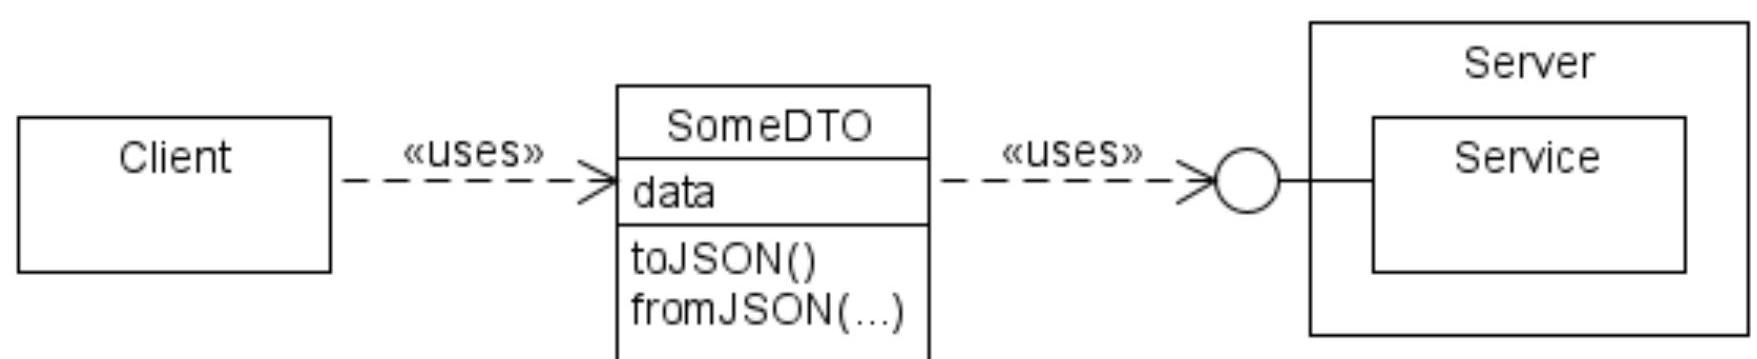
\includegraphics[width=\linewidth]{images/2025_01_02_9418c7c99690de3f1353g-18}
  \item Es bündelt mehrere Daten in einem Objekt, sodass sie durch einen einzigen Programmaufruf übertragen werden können.
  \item Der Zweck ist, mehrere zeitintensive Remotezugriffe durch einen einzigen zu ersetzen.
  \item Ein DTO ist in der Regel «immutable», d.h. enthält nur getter-Methoden.
\end{itemize}

\section*{Ausgewählte Implementierungsaspekte von Client-Server-Systemen}
\begin{itemize}
  \item Wir betrachten im Weiteren einige ausgewählte Aspekte:
  \item Heterogenität
  \item Serverarchitektur
  \item Nebenläufigkeit im Server (Parallelität)
  \item Serverseitige Service- bzw. Dienstschnittstellen
  \item Fehlersituationen, Fehlerklassierung
  \item Parameterübergabe zwischen Client und Server
  \item Marshalling/Unmarshalling
  \item Kommunikation
  \item Zustandsverwaltung
  \item Garbage Collection
  \item Lastverteilung, Verfügbarkeit, Skalierbarkeit
\end{itemize}

\section*{Heterogenität}
\begin{itemize}
  \item Mehrere Ebenen der Heterogenität
  \item Standardformate notwendig!
\end{itemize}

\section*{- Rechnerhardware und Betriebssysteme}
\begin{itemize}
  \item Unterschiede bei der Speicherung der Daten
  \item «Little Endian» versus «Big Endian»
  \item Unterschiedliche Zeichensätze
  \item ASCII - EBCDIC - Unicode\\
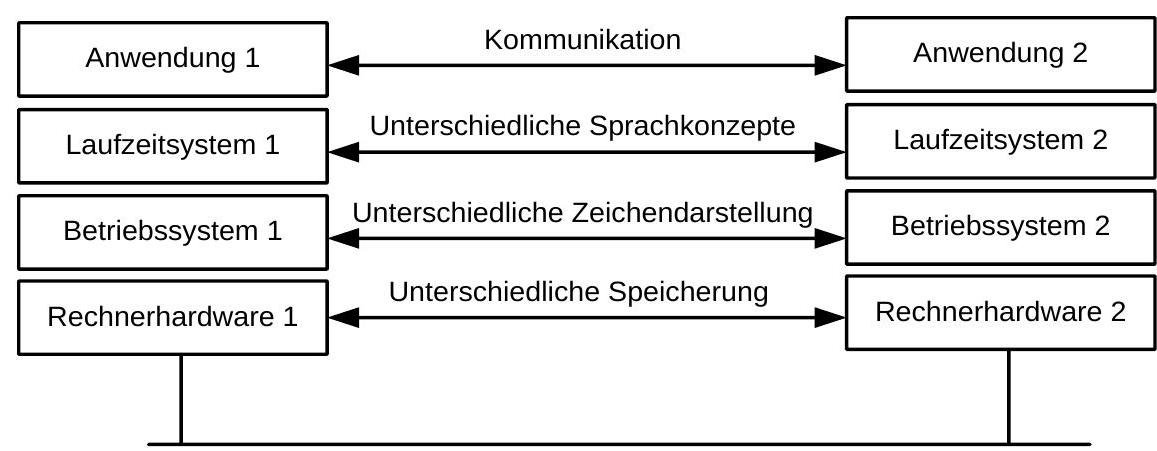
\includegraphics[width=\linewidth]{images/2025_01_02_9418c7c99690de3f1353g-20}
\end{itemize}

Darstellung: "little endian"\\
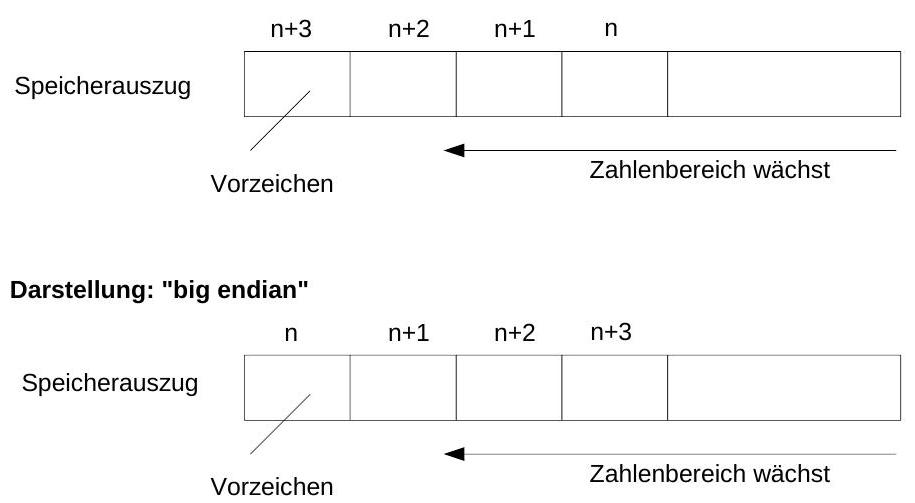
\includegraphics[width=\linewidth]{images/2025_01_02_9418c7c99690de3f1353g-20(1)}

\section*{Überlegungen zur Überwindung von Heterogenität}
\begin{itemize}
  \item Was wir brauchen!
  \item Einheitliche Transportsyntax (ASN.1, XDR, HTML, XML, JSON ...) $\rightarrow$ Schicht 6 (ISO/OSI-Modell)
  \item Middleware-Technologien bieten meist ähnliche Ansätze
  \item Marshalling (Serialisierung) und Unmarshalling (Deserialisierung) der Nachrichten über generierten Code (Stubs und Skeletons)\\
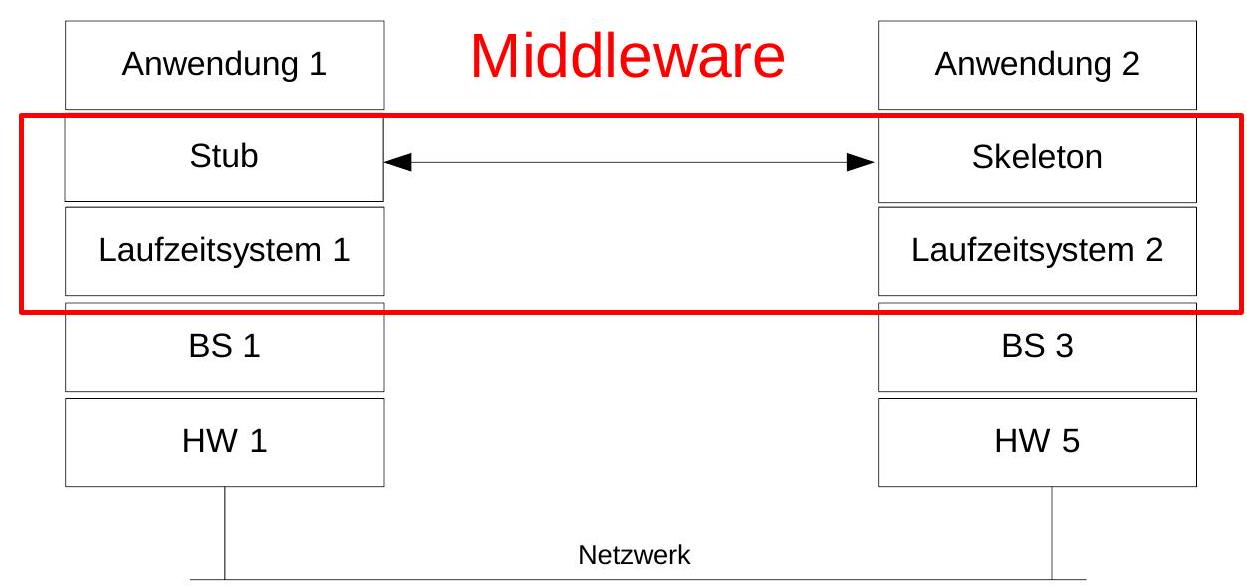
\includegraphics[width=\linewidth]{images/2025_01_02_9418c7c99690de3f1353g-21}
\end{itemize}

\section*{Nebenläufigkeit (Parallelität)}
\begin{itemize}
  \item Iterative (sequentielle) oder parallele Serverbausteine
  \item Threadpooling, Multithreading für die Bedienung mehrerer Clients gleichzeitig
  \item Ein Dispatcher ist ein Softwarebaustein im Server, der alle Requests der Clients entgegennimmt und sie auf Threads verteilt
  \item Einfaches sequentielles Programmiermodell für die Programmierer-Sicht
  \item Im JDK gibt es verschiedene Klassen für Thread-Pooling (s. java.util.concurrent)\\
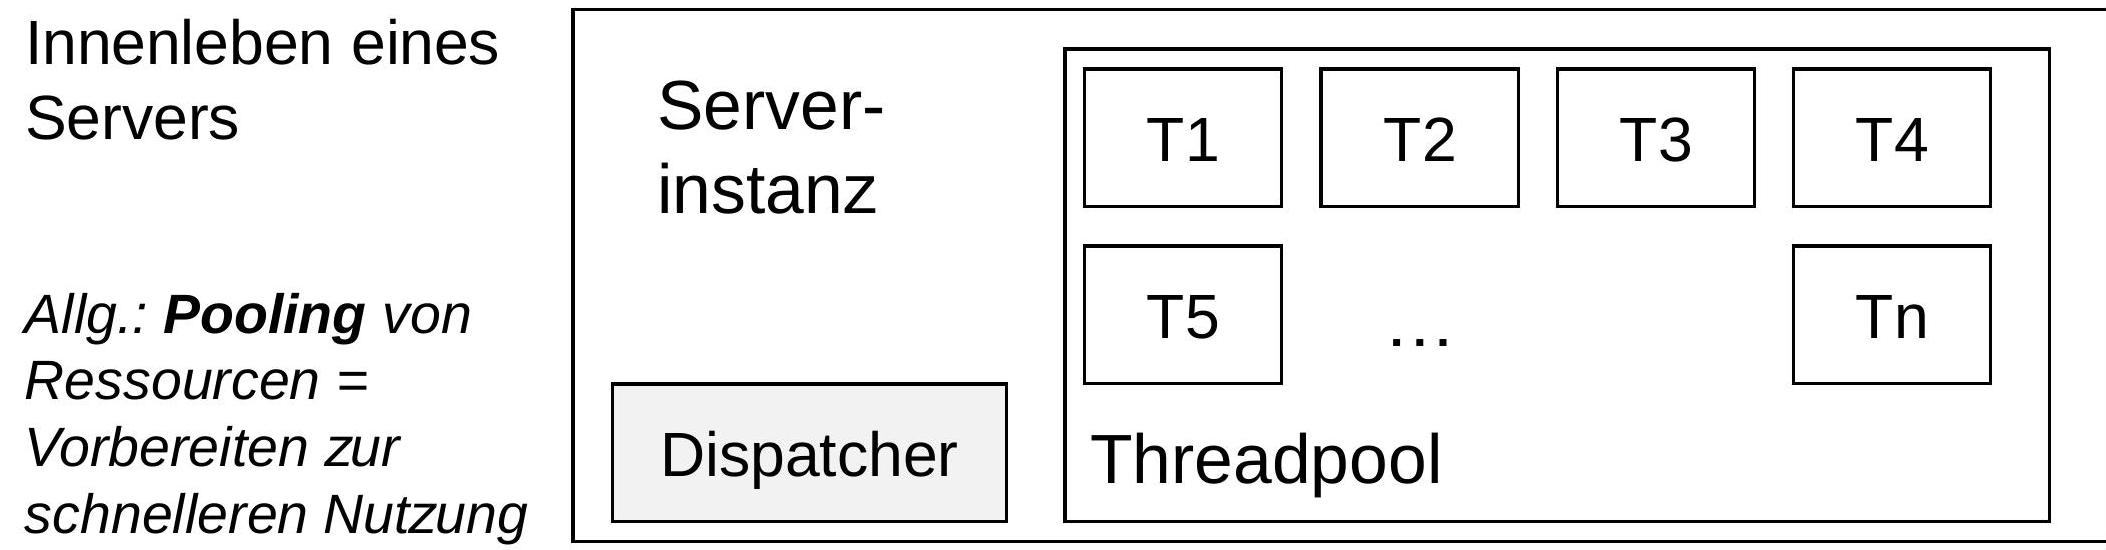
\includegraphics[width=\linewidth]{images/2025_01_02_9418c7c99690de3f1353g-22}
\end{itemize}

\section*{Dienst- bzw. Serviceschnittstellen}
\begin{itemize}
  \item Wie wird die Schnittstelle (Parameter- und Rückgabewertetypen) eines Serverbausteins beschrieben?
  \item Neutrale Schnittstellenbeschreibungssprache oder eingebettet in Hostsprache (sprachabhängig)
  \item Exception-Behandlung nicht immer gleich
  \item Diskussionsfrage:
  \item Wie gut muss ein Server, der einen Service bereitstellt, prüfen, ob die empfangenen Parameter korrekt sind?
\end{itemize}

\section*{Fehlersituationen}
\begin{itemize}
  \item Es kann u.a. passieren, dass
  \item ein Auftrag (engl. request) verloren geht,
  \item das Ergebnis (engl. reply) des Servers verloren geht,
  \item der Server während der Ausführung des Auftrags abstürzt,
  \item der Server für die Bearbeitung des Auftrags zu lange braucht oder
  \item der Client vor Ankunft des Ergebnisses abstürzt.\\
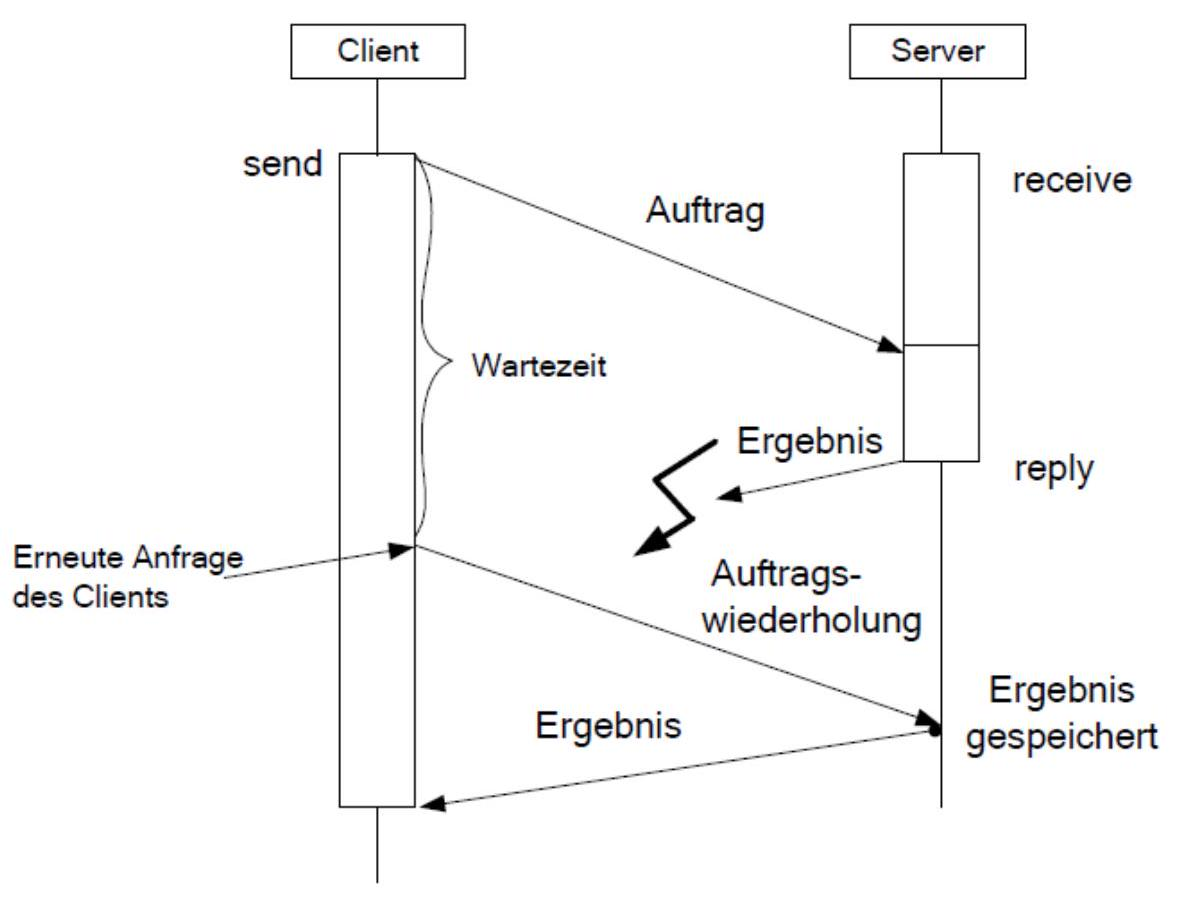
\includegraphics[width=\linewidth]{images/2025_01_02_9418c7c99690de3f1353g-24}
\end{itemize}

\section*{Parameterübergabe}
\begin{itemize}
  \item Methodenaufruf und Parameterübergabe
  \item ist lokal in demselben Prozess einfacher als bei entferntem (remote) Aufruf.
  \item Entfernte Methodenaufrufe müssen für die Datenübertragung zwischen Rechnerknoten serialisiert (Marshalling) und deserialisiert (Unmarshalling) werden.
  \item Varianten für den entfernten Aufruf:
  \item Call-by-value: Wert wird übergeben
  \item Synonym: Call-by-copy
  \item Call-by-reference: Verweis auf Variable wird übergeben
  \item Call-by-copy/copy-back: Aufrufer arbeitet mit Kopie
  \item Synonym: Call-by-restore = Call-by-value-result
\end{itemize}

\section*{Marshalling/Unmarshalling}
\begin{itemize}
  \item Marshalling/Unmarshalling ist das Umwandeln (Serialisierung/Deserialisierung) von strukturierten oder elementaren Daten für die Übermittlung an andere Prozesse.
  \item Tag-basierte Transfersyntax
  \item Siehe ASN. 1 mit BER (Basic Encoding Rules)
  \item TLV-Kodierung (Type, Length, Value)
  \item Tag-freie Transfersyntax
  \item Siehe Sun ONC XDR, CORBA CDR
  \item Beschreibung der Daten aufgrund der Stellung in der Nachricht
  \item Aufbau der Datenstrukturen ist dem Sender und dem Empfänger bekannt
  \item Meist automatische Erzeugung von Marshalling- und Unmarshalling-Routinen durch Compiler/Präcompiler
  \item Heute werden oft auch sprachunabhängige Notationen verwendet:
  \item XML (Markup-Sprache), Tag-basiert
  \item JSON (JavaScript Object Notation), Tag-basiert, sprachunabhängig?
\end{itemize}

\section*{Kommunikationsmodelle: Synchrone Kommunikation}
School of

\begin{itemize}
  \item Synchroner entfernter Dienstaufruf $\rightarrow$ blockierend
  \item Der Sender wartet, bis eine Methode send mit einem Ergebnis zurückkehrt\\
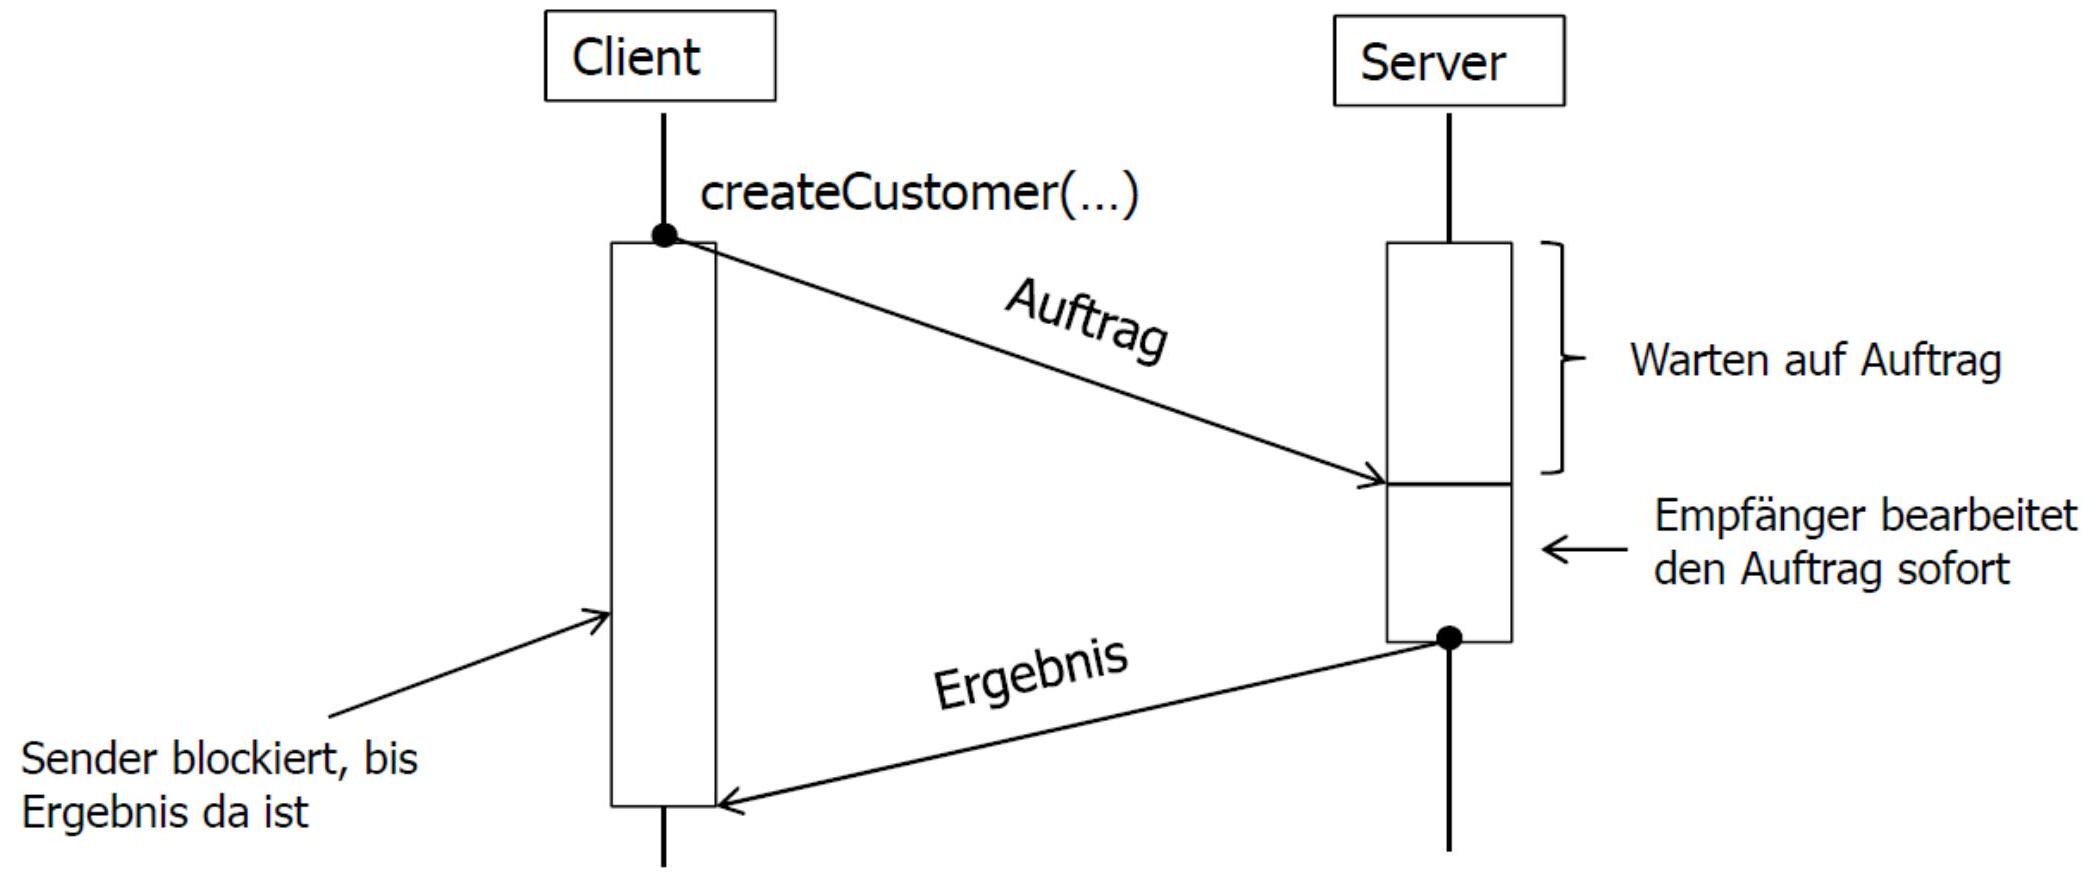
\includegraphics[width=\linewidth]{images/2025_01_02_9418c7c99690de3f1353g-27}
\end{itemize}

Synchronisation = Synchronisierung (griech: sýn = zusammen, chrónos = Zeit): Aufeinander-Abstimmen von Vorgängen (zeitlich). Engere Bedeutung je nach Wissensgebiet: siehe Film, Informatik,...

\section*{Kommunikationsmodelle: \\
 Asynchrone Kommunikation}
\begin{itemize}
  \item Asynchroner entfernter Serviceaufruf $\rightarrow$ Nicht blockierend, der Sender kann weiter machen\\
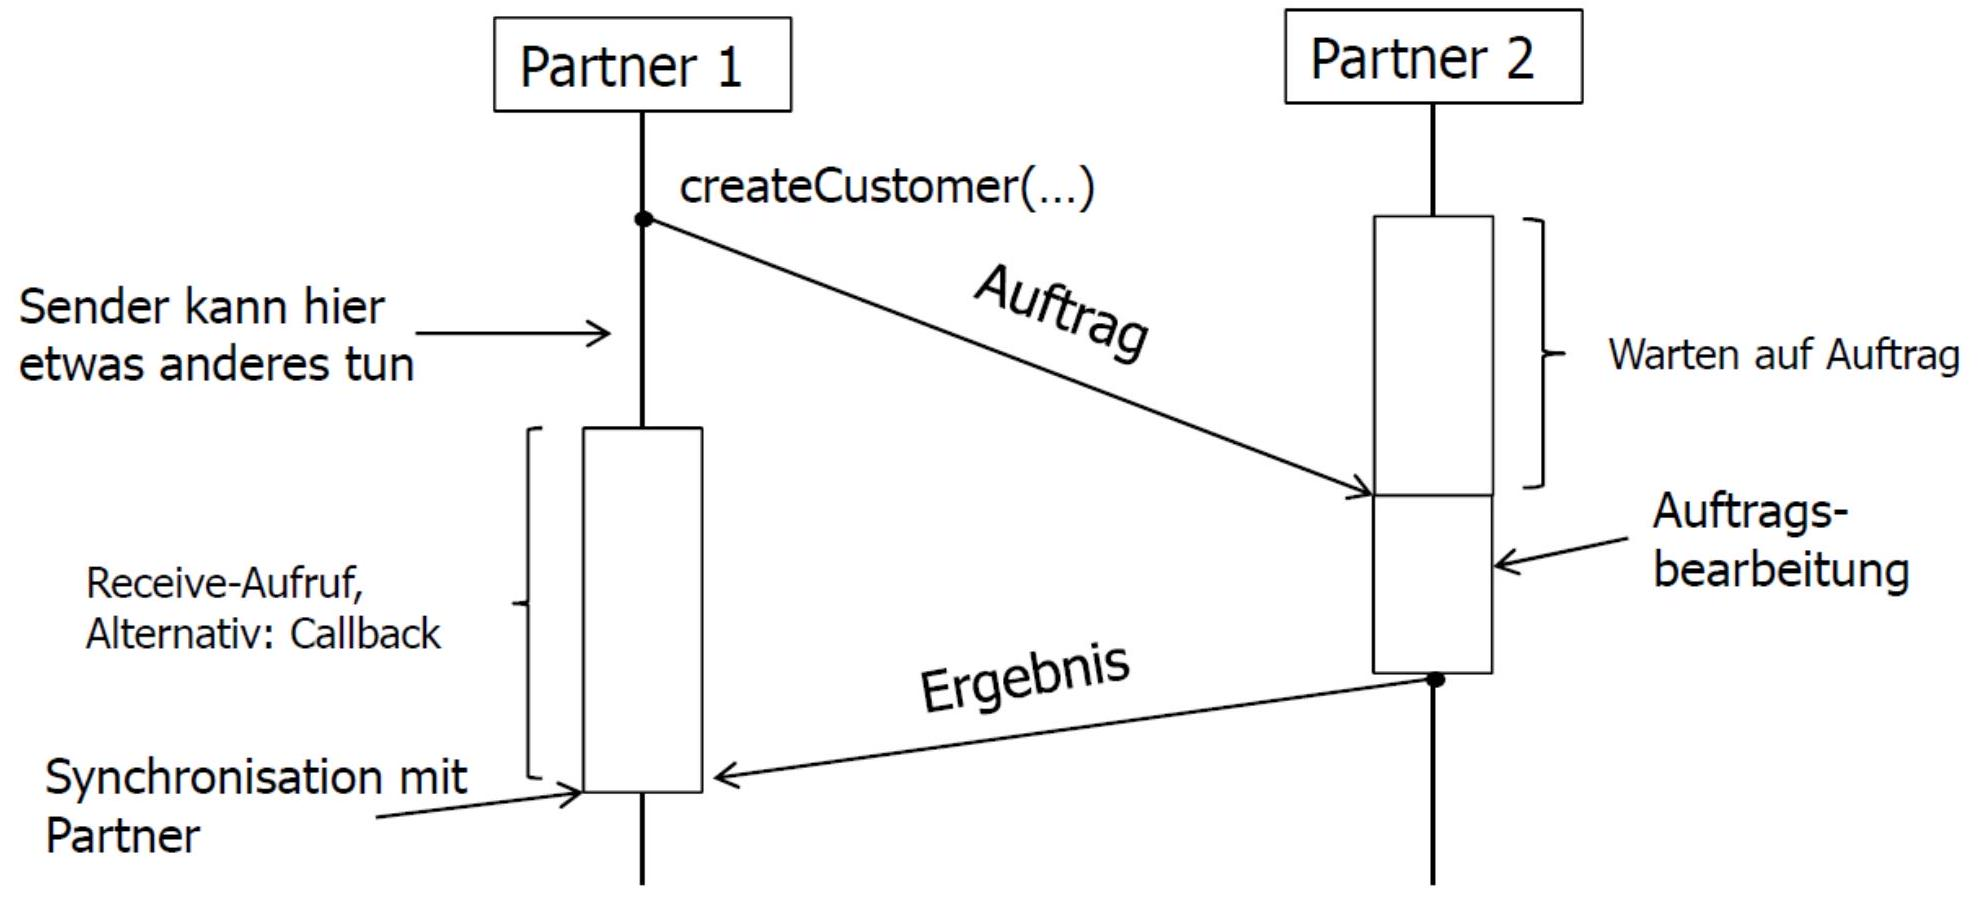
\includegraphics[width=\linewidth]{images/2025_01_02_9418c7c99690de3f1353g-28}
\end{itemize}

In der Datenkommunikation: asynchron = Senden und Empfangen von Daten zeitlich versetzt und ohne Blockieren des Prozesses

\section*{Kommunikation}
\begin{itemize}
  \item Namensauflösung und Adressierung auf der Anwendungsebene (entferntes Objekt oder Prozedur)
  \item Naming- und Directory-Services notwendig
  \item Binding-Vorgang: Aufbau eines Verbindungskontextes zwischen Client und Server
  \item Statisch zur Übersetzungszeit
  \item Dynamisch zur Laufzeit
  \item Kommunikationsprotokoll für die Client-Server-Kommunikation
  \item Nachrichtentypen (meist Request-Response-Protokolle)
  \item Unterstützte Fehlersemantik
  \item Unterstützung für verteiltes Garbage Collection
\end{itemize}

\section*{Zustandsverwaltung}
\begin{itemize}
  \item Server können zustandsinvariante und zustandsändernde Dienste bzw. Services anbieten
  \item Zustandsändernde Dienste führen bei der Bearbeitung zu einer Änderung von Daten (z.B. in Datenbanken)
  \item Zustandsinvariante Dienste verändern nichts
  \item Weiterer Aspekt: Server muss sich das Wissen über die Zustandsänderung über einen Aufruf hinweg merken
  \item stateful und stateless Server
  \item Stateless Server verwalten den aktuellen Zustand der Kommunikationsbeziehung zwischen Client und Server nicht
  \item Wenn möglich: stateless!
  \item Zustandslose Kommunikationsprotokolle im Web: HTTP und REST für Webservices
\end{itemize}

\section*{Garbage Collection (GC)}
\begin{itemize}
  \item Verteiltes Reference-Counting
  \item Server verwaltet eine Liste aller Clients (Proxies), die entfernte Referenzen nutzen
  \item Server verwaltet Referenzzähler für alle benutzten Objekte
  \item Client sendet spezielle Nachrichten an den Server, wenn Referenz benutzt bzw. gelöscht wird
  \item Leases
  \item Referenz wird nur eine begrenzte Zeit für den Client freigegeben
  \item Nach definierter Zeit löscht der Server die Referenz, wenn sich der Client nicht meldet
  \item Ein Client kann sich somit problemlos beenden
  \item Zusammenarbeit mit lokalen GC-Mechanismen
  \item Heap-Bereinigung
\end{itemize}

\section*{Lastverteilung, Hochverfügbarkeit, Skalierbarkeit}
\begin{itemize}
  \item Load Balancing (Lastverteilung)
  \item Lastverteiler verteilen die Last auf mehrere Serverinstanzen
  \item Dispatching z.B. über DNS-basiertes Request-Routing
  \item Hochverfügbarkeit
  \item Server-Cluster, Beispiel: JBoss Cluster, Oracle Real Application Cluster
  \item Failover
  \item Session-Replikation
  \item Skalierbarkeit
  \item Horizontal: Steigerung der Leistung durch Hinzunahme von Rechnern
  \item Vertikal: Steigerung der Leistung durch Hinzufügen von Ressourcen zu einem Rechner (CPU, Speicher, ...)
\end{itemize}

\begin{enumerate}
  \item Einführung in verteilte Systeme
  \item Design- und Implementierungskonzepte von Client/Server-Systemen
  \item Middleware für verteilte Systeme
  \item Wrap-up und Ausblick
\end{enumerate}

\begin{itemize}
  \item Middleware ist eine Softwareschicht, die den Anwendungen standardisierte, höhere Kommunikationsund sonstige Dienste über ein Application Programming Interface (API) bereitstellt und damit die transparente\\
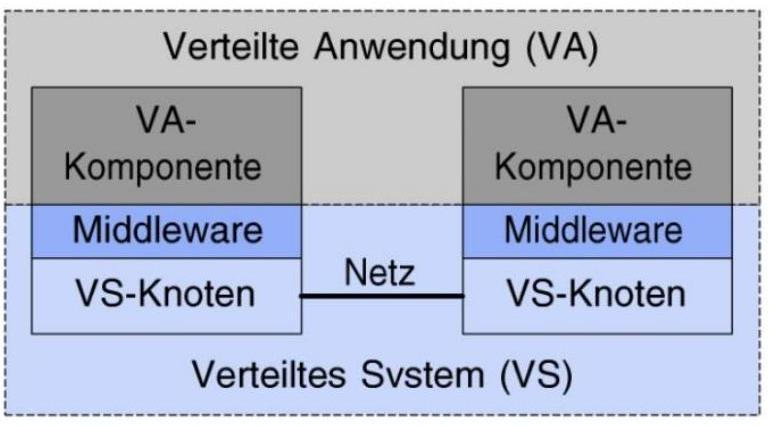
\includegraphics[width=\linewidth]{images/2025_01_02_9418c7c99690de3f1353g-34} Kommunikation von Komponenten verteilter Systeme unterstützt.
\end{itemize}

\section*{- Anwendungsorientierte Middleware}
 Java Enterprise Edition (EE) neu Jakarta EE\begin{center}

\includegraphics[width=\linewidth]{images/2025_01_02_9418c7c99690de3f1353g-35}
\end{center}

Anwendungs-\\
komponente Anwendungskomponente komponente Komponentenmodell Dienste Laufzeitumgebung Dienste\\
Kommunikationsinfrastruktur\\
Betriebssystem / Verteiltes System\\
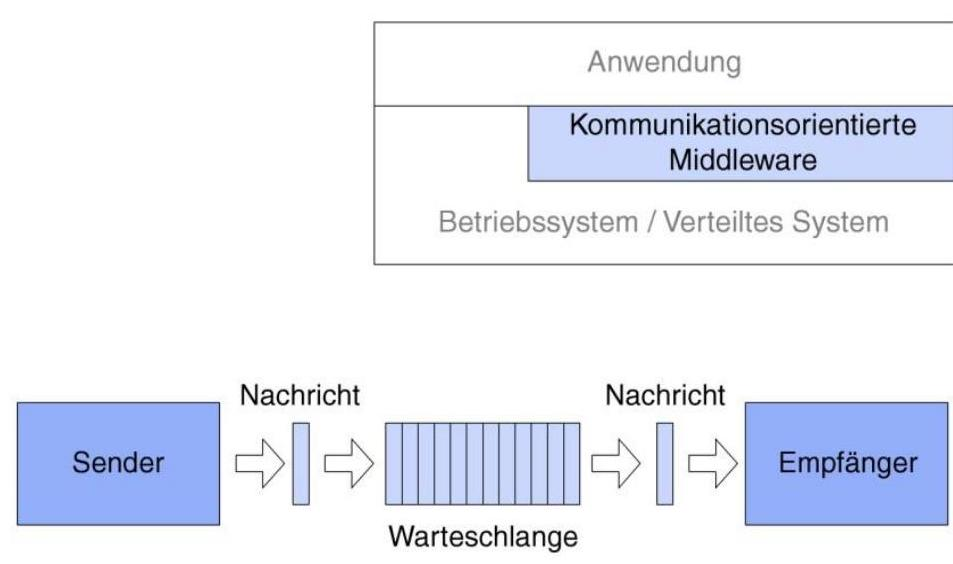
\includegraphics[width=\linewidth]{images/2025_01_02_9418c7c99690de3f1353g-35(1)}

\begin{itemize}
  \item Kommunikationsorientierte Middleware Remote Procedure Call (RPC), Remote Method Invocation (RMI), REST, WebSocket ...
  \item Nachrichtenorientierte Middleware Message Oriented Middleware (MOM), Java Messaging Service (JMS), MQTT ...
\end{itemize}

Implementierungskonzepte:\\
Konkrete Ansätze für das Client-Server-Modell

\begin{itemize}
  \item Remote Procedure Call (RPC)
  \item z.B. Sun ONC RPC, DCE RPC
  \item Verteilte Objekte
  \item z.B. CORBA, Java RMI, .NET Remoting
  \item Verteilte Services
  \item z.B. Webservices, SOAP, RESTful
\end{itemize}

\section*{Implementierungskonzepte: \\
 Konkrete Ansätze für das Client-Server-Modell}
\begin{itemize}
  \item Auf den folgenden Folien finden Sie verschieden Implementierungsansätze zu verschiedenen Ebenen der Programmierung.
  \item Socket
  \item RPC (remote procedure call)
  \item RMI (remote method invocation) -> mit Fallstudie
  \item Web-basierte Kommunikation, angewendete Protokolle
  \item Websockets -> mit Fallstudie
  \item Web-Services -> mit Fallstudie REST (Representational State Transfer)
\end{itemize}

\begin{enumerate}
  \item Einführung in verteilte Systeme
  \item Design- und Implementierungskonzepte von Client-Server-Systemen
  \item Middleware für verteilte Systeme
  \item Wrap-up und Ausblick
\end{enumerate}

\begin{itemize}
  \item Ein verteiltes System setzt sich aus einzelnen voneinander unabhängigen Bausteinen (Komponenten) zusammen, die dem Benutzer wie ein einzelnes kohärentes System erscheinen.
  \item Verteilte Systeme sind komplizierter als nicht verteilte Systeme und es müssen verschiedene praktische Probleme gelöst werden (Heterogenität, Fehlersituationen, Deployment etc.).
  \item Gängige Architekturstile verteilter Systeme sind Client-Server, Peer-to-Peer und Event Systems.
  \item Wichtige Design- und Implementierungsaspekte von Client-Server-Systemen sind RequestHandling (Threading), Design der serverseitigen Serviceschnittstellen, unterstützte Fehlersemantik, Parameter-Übergabe (Call-by-value, Call-by-reference), Kommunikationsstil (synchron, asynchron), Zustandsverwaltung und Garbage Collection.
  \item Grundlegende Architektur und Design Patterns für verteilte Systeme sind: Remote Proxy, Service Locator, Data Transfer Object und Remote Facade.
  \item Java RMI (Remote Method Invocation) ist die objektorientierte Umsetzung des RPCs (Remote Procedure Call) in Java und realisiert einen transparenten, entfernten Methodenaufruf.
  \item Web-basierte Applikationen verwenden das zustandslose Protokoll HTTP(S), Ajax und RESTful Webservices für die Kommunikation zwischen Browser und Webserver.
\end{itemize}

\section*{Ausblick}
\begin{itemize}
  \item In der nächsten Lerneinheit werden wir:
  \item das Thema GUI-Architekturen vertiefen.
\end{itemize}

\section*{Quellenverzeichnis}
[1] Mandl, P.: Masterkurs Verteilte betriebliche Informationssysteme, Springer-Vieweg, 2008\\[0pt]
[2] Schill, A.; Springer, T.: Verteilte Systeme, 2. Auflage, Springer-Vieweg, 2012\\[0pt]
[3] Fowler, M.: Patterns of Enterprise Application Architecture, Addison Wesley, 1. Auflage, 2002\\[0pt]
[4] Martin, R. C.: Clean Architecture: A Craftsman's Guide to Software Structure and Design, mitp Professional, 2018\\[0pt]
[5] Abts D.: Masterkurs Client/Server Programmierung mit Java, 5. Auflage, Springer-Vieweg, 2019


\end{document}